%!TEX root = ../Thesis.tex
\section{Planar Intersection Algorithm}


https://www.e-education.psu.edu/geog862/node/1759 - errors in pseduorange

http://www.insidegnss.com/node/2898 - how to get pseudorange from raw data


\paragraph{Select reference receiver}
The receiver $\alpha$ is used as the reference location and common epoch time. The reference location is calculated by performing NLLS on a receiver to calculate the absolute position for one point in time. Any receiver can be used as the reference point. For a real world implementation, all of the raw data can be sent to each node and it uses itself as the reference point.
\paragraph{Collect data of one timestep from all receivers}
The raw data as well as the estimated absolute location and clock bias (what frame of reference is this?) from non-linear least squares optimisation is collected from all GPS receivers.
\paragraph{Align to reference Epoch time}\label{timetransform}


%\subsubsection{Distance Optimisation}
%By optimising the distance between each pair of receivers, the error in the whole system is minimised. 
%This means that the position receivers are not only relative to the reference receiver $\alpha$ but between all receivers just with the reference frame origin located at $\alpha$. It is because of this step a receiver does not need to have all the same satellites in view as all other receivers, including the designated $\alpha$.


\paragraph{Average normal Vector}
Find the average normal vector pointing to each satellite $\hat{\eta_s}$ from the receivers. The normal vector is calculated by using the position all of the satellites in view at the common time $t_{\alpha}$ as previously transformed in \ref{timetransform} and the estimated absolute position of all receivers. The average for each satellite is calculated by taking the mean across all receivers.

\paragraph{Difference in Pseudorange}
The differences in pseudorange are calculated $\Omega^s_\omega$ in the ECEF frame where s is the satellite, $\omega$ is the receiver.

\paragraph{Create Planes}
Sets of planes are created for each receiver $\omega$. The equation of a plane is $Ax+By+Cz+D=0$ where the coefficients [A,B,C] describe the normal vector of the plane and the coefficient D sets the plane in 3D space along the vector, Eq\eqref{genplane}. As the normal vector is already calculated for each satellite, only the D coefficient must be solved for each receiver and satellite pair. 
\begin{eqnarray}
P_\omega^s &:& (\textbf{i}\cdot\hat{\eta_s})x + (\textbf{j}\cdot\hat{\eta_s})y + (\textbf{k}\cdot\hat{\eta_s})z + D_\omega^s \label{genplane} = 0
\end{eqnarray}

\paragraph{Solve for D}
The coefficient D is calculated by finding a point on the plane $f_\omega^s$, then substituting it into Eq\eqref{genplane} for x,y,z; Eq\eqref{Eq:solvef}. The point of the plane is calculated by moving along the normal vector by the difference in pseudorange from the reference point Eq\eqref{Eq:f}, see Figure \ref{fig:solvef}.
\begin{eqnarray}
f_\omega^s &=& -\Omega_\omega^s\hat{\eta_s} \label{Eq:f}
\end{eqnarray}

\begin{figure}[t]
\centering
\caption{Construction of Planes}
\label{fig:solvef}
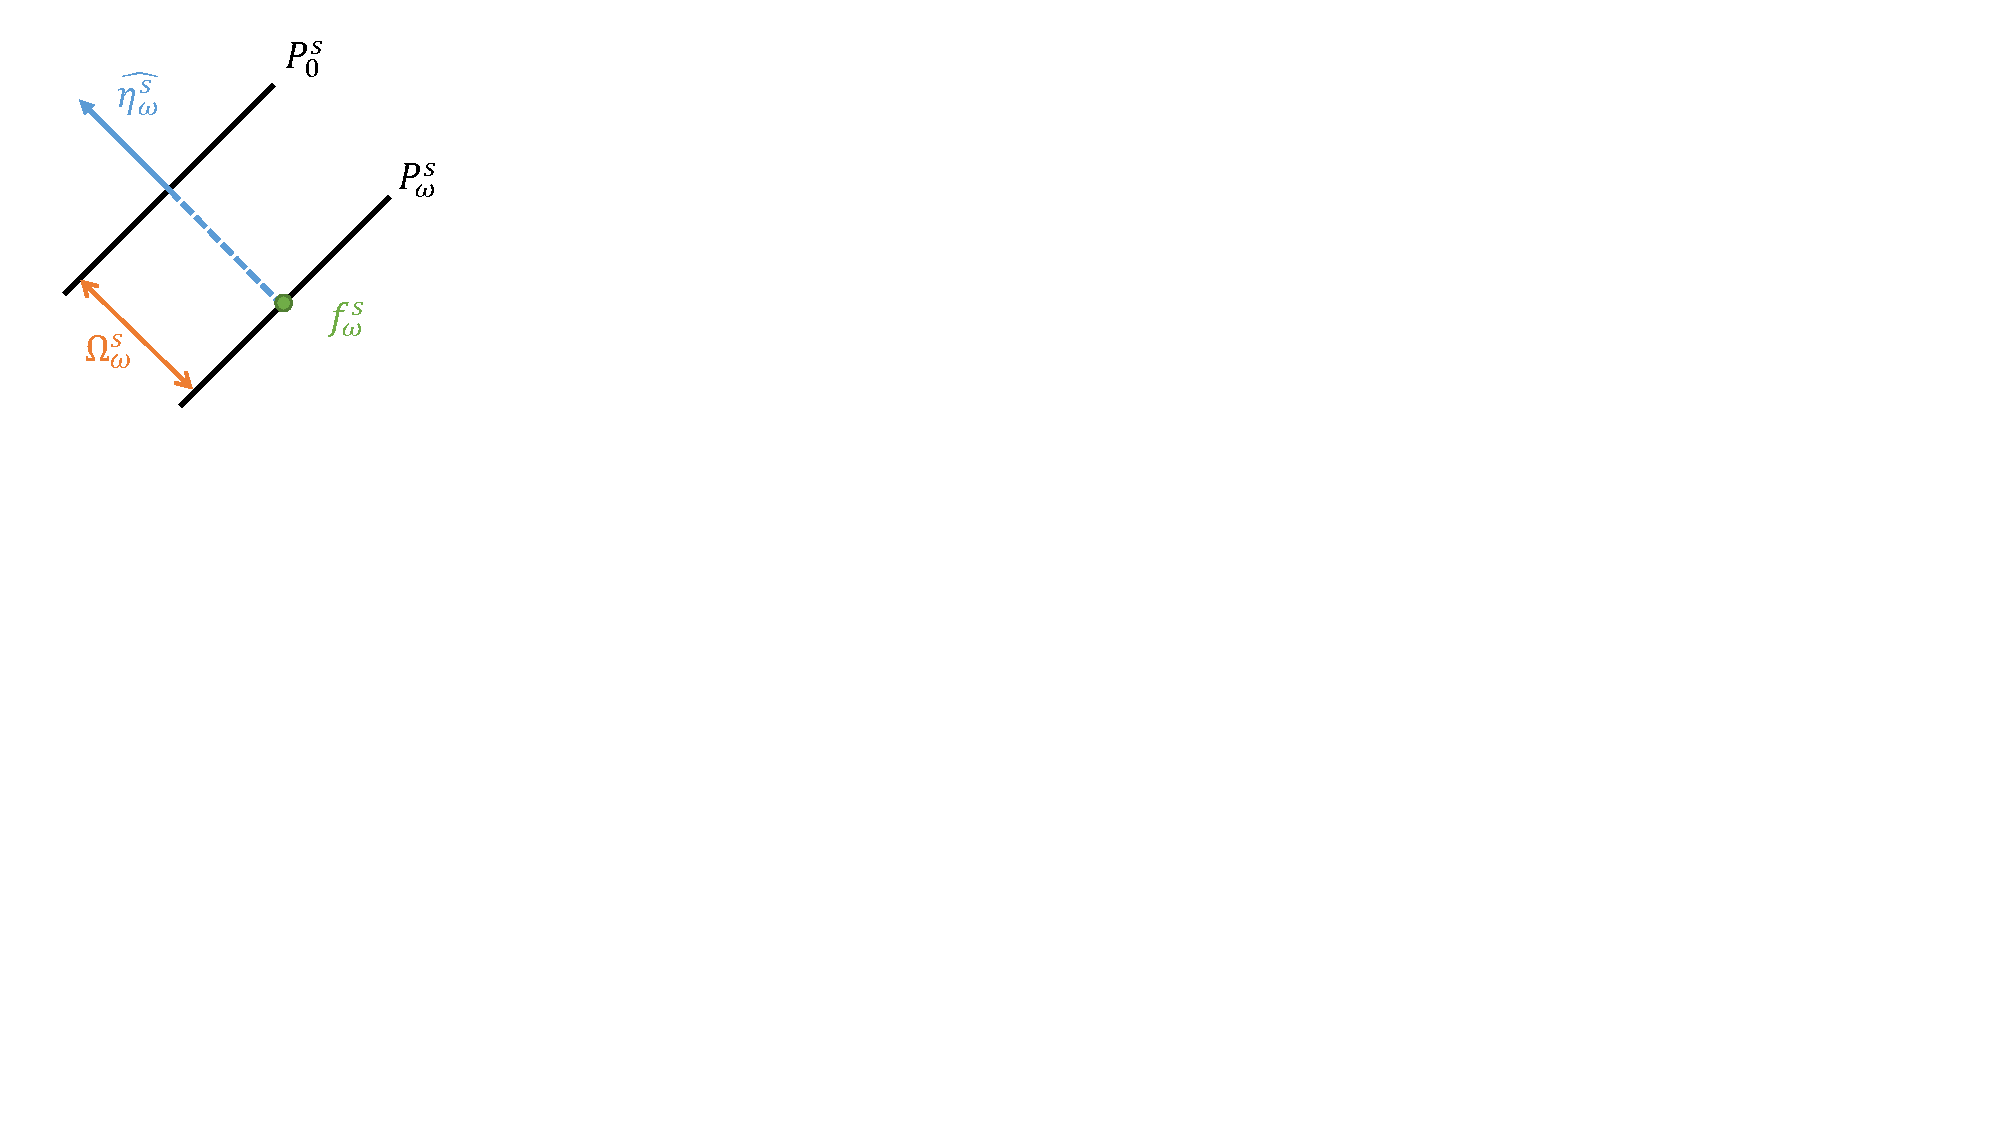
\includegraphics[trim=0 12cm 26cm 0,clip,width =0.6\linewidth]{ChapterPerception/Figures/solveF.pdf}
\end{figure}

As the algorithm is solved in 3D space relative to the reference receiver (the origin is the reference receiver), the coefficient D is actually the measured difference in pseudorange $\Omega^s_{\omega}$. The following is the proof.
 
\begin{eqnarray}
\hat{\eta_s}\cdot f_\omega^s + D_\omega^s &=& 0 \label{Eq:solvef}\\
D_\omega^s &=& -\hat{\eta_s}\cdot f_\omega^s \nonumber\\
D_\omega^s &=& -\hat{\eta_s}\cdot (-\Omega_\omega^s\hat{\eta_s}) \nonumber\\
D_\omega^s &=& \Omega_\omega^s ||\hat{\eta_s}||^2 \nonumber\\
as \;||\hat{\eta_s}|| &=& 1 \nonumber\\
D_\omega^s &=& \Omega_\omega^s
\end{eqnarray}


\paragraph{Solve for Intersection}
Four variables for each receiver must be solved for $X_\omega = [x,y,z,\tau]^T$. The vector $X_\omega$ describes the position of receiver $\omega$ in NED coordinates and $\tau_\omega$ describes a final receiver clock bias that alters the displacement of all the planes in the set $P_\omega$ by the same parameter. 

In order to solve all of the receivers with the least amount of error in the whole system, all of the position vectors $X_\omega$ are solved at the same time. The reference planes of $\alpha$ must be included as a constraint on the system. All of the clock biases are also constrained with the clock bias from $\tau_\alpha$, see \eqref{Eq: P with alphat}. The receiver clock bias only affects the equation of the planes by altering the constant as a change in the pseudorange has no affect over the angle of the plane. Each receiver clock bias alters all the planes associated with that receiver proportionally. 
\begin{eqnarray}
(\textbf{i}\cdot\hat{\eta_s})(x-x_0) + (\textbf{j}\cdot\hat{\eta_s})(y-y_0) + (\textbf{k}\cdot\hat{\eta_s})(z-z_0) + (\tau_\omega-\tau_0) = -\Omega_\omega^s \label{Eq: P with alphat}
\end{eqnarray} 
In matrix form, one 
\begin{equation}
 \left[ \hat{\eta_s}, 1 \right] \times [X_\omega - X_0] = -\Omega_\omega^s
\end{equation}

The matrix N (4 x n) is describes the set of normal vectors to all of the satellites $s\in\{1...n\}$
\begin{equation}
N = \begin{bmatrix}
\hat{\eta_1} & 1\\
\hat{\eta_2} & 1 \\
\vdots & \vdots \\
\hat{\eta_n} & 1
\end{bmatrix}
\end{equation}

$G_\omega$ is a n x 1 matrix that contains all of the difference in pseudoranges between the reference receiver and the receiver $\omega$ for all satellites $s\in\{1...n\}$
\begin{equation}
G_\omega = \begin{bmatrix}
\Omega_\omega^1 \\
\Omega_\omega^2 \\
\vdots\\
\Omega_\omega^n
\end{bmatrix}
\end{equation}
There are m+1 receivers in the system, therefore the total set of distances encompasses   $G_\omega$ for $\omega\in\{1...m\}$ where $G_0$ is the empty set that constrains the position of the reference receiver and constrains the system to the relative frame.

\begin{eqnarray}
\begin{bmatrix}
N & \{0\} & \hdotsfor{1} &\{0\} \\
-N & N  &\{0\} &  \hdotsfor{1} \\
\vdots & \{0\}  & \ddots & \{0\} \\  
-N & \{0\} &  \hdotsfor{1}& N
\end{bmatrix} 
\begin{bmatrix}
X_0 \\
X_1 \\
\vdots \\
X_m
\end{bmatrix} &=& 
\begin{bmatrix}
G_0 \\
G_1 \\
\vdots \\
G_m
\end{bmatrix}\\
\Phi\chi &=& \Gamma
\end{eqnarray}

As the number of satellites each receiver can see can be 4 or more, the system is overdetermined. An overdetermined system is solved by least squares. That is, there is a solution that minimises the residuals $||\Phi\chi-\Gamma||^2$ by using the pseudo-inverse of $\Phi$:
\begin{eqnarray}
\chi = (\Phi^T\Phi)^{-1}\Phi^T\Gamma
\end{eqnarray}

\paragraph{Limitations}
The pseudo-inverse requires that the matrix equations be linearly independent. Therefore the satellite configuration cannot have two satellites at the same location. Also, all of the satellites cannot have the exact same elevation or azimuth as the inverse approaches singularity which introduces error based on the mathematical instability. In reality it is extremely unlikely that these configurations would occur, but it does effect the satellite configurations analysis in the next Chapter.



